\documentclass[usenames, dvipsnames, aspectratio = 169, 13pt]{beamer}

\usepackage{color}
% Typesetting
	\usepackage{amsfonts}
	\usepackage{amssymb}
	\usepackage{amsmath}

	\usepackage{subfig}

	\usepackage{graphicx}
    
    \usepackage{multicol}
    \usepackage{tikz}
    \usetikzlibrary{calc,intersections}
    
    \usepackage{dcolumn}
    
    \usepackage{accents}
    \usepackage{adjustbox}

% Bibliography
    % \usepackage[style=authoryear-comp,natbib=true,backend=biber]{biblatex}
    % \addbibresource{Bibliography.bib}
    % \usepackage{csquotes}
	\usepackage{natbib}
 	%\bibliographystyle{apalike}
 	\bibliographystyle{aer}
	
	\usepackage{bibunits}
	\defaultbibliography{Bibliography.bib}  
	%\defaultbibliographystyle{apalike}
	\defaultbibliographystyle{aer}

	
% Links
	\usepackage{hyperref}
	\hypersetup{
    colorlinks=true,
    linkcolor=black,
    filecolor=magenta,      
    urlcolor=blue,
    citecolor = black
}
	\usepackage{cleveref}

% Todonotes
	\usepackage[framemethod=tikz]{mdframed}
	\usepackage{todonotes}
	\presetkeys{todonotes}{color=black!5,inline}{} % noline

% Boxes
    \usepackage{tcolorbox}
    \newtcbox{\feedback}{nobeforeafter,colframe=black,colback=white,boxrule=0.5pt,arc=2pt,
      boxsep=0pt,left=2pt,right=2pt,top=2pt,bottom=2pt,tcbox raise base}
      
% Theorems
    \usepackage{amsthm}
     
    \newtheorem{thm}{Theorem}
    \newtheorem{asm}{Assumption}
    \newtheorem{con}{Conjecture}
    \newtheorem{prop}{Proposition}
    \newtheorem{lem}{Lemma}
    \newtheorem{cor}{Corollary}
    \newtheorem{rem}{Remark}
    \newtheorem{defn}{Definition}

%Packages and commands for column widths in tables
\usepackage{array}
\newcolumntype{L}[1]{>{\raggedright\let\newline\\\arraybackslash}m{#1}}
\newcolumntype{C}[1]{>{\centering\let\newline\\\arraybackslash\hspace{0pt}}m{#1}}
\newcolumntype{R}[1]{>{\raggedleft\let\newline\\\arraybackslash\hspace{0pt}}m{#1}}

%Turn off toolbar
\setbeamertemplate{navigation symbols}[default]
\beamertemplatenavigationsymbolsempty  


%Macro for wrapping text in underbrace
\usepackage{ragged2e}
\newlength\ubwidth
\newcommand\wrapunderbrace[2]{\settowidth\ubwidth{$#1$}\underbrace{#1}_{\parbox{\ubwidth}{\scriptsize\RaggedRight#2}}}


%This makes citations smaller
\makeatletter
\DeclareRobustCommand\citep
{\begingroup\footnotesize\NAT@swatrue\let\NAT@ctype\z@\NAT@partrue
    \@ifstar{\NAT@fulltrue\NAT@citetp}{\NAT@fullfalse\NAT@citetp}}
\makeatother
% Probability
\renewcommand{\P}{\mathop{}\!\textnormal{P}}
\newcommand{\E}{\mathop{}\!\textnormal{E}}
\newcommand{\sE}{\mathop{}\!\mathbb{E}}
\newcommand{\Cov}{\mathop{}\!\textnormal{Cov}}
\newcommand{\sCov}{\mathop{}\!\mathbb{C}\textnormal{ov}}
\newcommand{\Var}{\mathop{}\!\textnormal{Var}}
\newcommand{\sVar}{\mathop{}\!\mathbb{V}\textnormal{ar}}
\newcommand{\N}{\mathcal{N}}
\newcommand{\sN}{\N(0,1)}

\newcommand{\bracks}[1]{\left[#1\right]}
\newcommand{\expe}[1]{\mathbb{E}\bracks{#1}}
\newcommand{\expestar}[1]{\mathbb{E}^*\bracks{#1}}
\newcommand{\expesub}[2]{\mathbb{E}_{#1}\bracks{#2}}

\newcommand{\var}[1]{\mathbb{V}\text{ar}\bracks{#1}}
\newcommand{\parens}[1]{\left(#1\right)}
  \newcommand{\squared}[1]{\parens{#1}^2}
  \newcommand{\tothepow}[2]{\parens{#1}^{#2}}
  \newcommand{\prob}[1]{\mathbb{P}\parens{#1}}
  \newcommand{\probsub}[2]{\mathbb{P}_{#1}\parens{#2}}

% Convergence
\newcommand{\Oh}{\mathop{}\!\mathcal{O}}
\newcommand{\oh}{\mathop{}\!{o}}
\newcommand{\convd}{\stackrel{d}{\longrightarrow}}
\newcommand{\convp}{\stackrel{p}{\longrightarrow}}
\newcommand{\conv}{\stackrel{}{\longrightarrow}}

% Basic matrices and vectors
\newcommand{\0}{\mathbf{0}}
\newcommand{\1}{\mathbf{1}}
\newcommand{\I}{\mathbb{I}}
\renewcommand{\O}{\mathbb{O}}

% Basic maths
\newcommand{\R}{\mathbb{R}}
\DeclareMathOperator*{\argmin}{arg\,min}
\DeclareMathOperator*{\argmax}{arg\,max}
\newcommand{\Ind}{\mathbbm{1}}  % Indicator
\newcommand{\reals}{\mathbb{R}}
% Estimation specifics
  \newcommand{\Ih}{\widehat{I}}
  \newcommand{\Is}{\mathcal{I}}
  
% Independence
  \newcommand{\orth}{\perp}
  \renewcommand{\given}{\: | \:}
  
% Prediction
\newcommand{\X}{\mathcal{X}}  % Covariate space
\newcommand{\W}{\mathcal{W}}  % Transformed covariate space
\newcommand{\Y}{\mathcal{Y}}  % Outcome space
\newcommand{\err}{\varepsilon}  % Outcome error
\newcommand{\g}{g}  % Truth (conditional expectation/optimal predictor)
\newcommand{\F}{\mathcal{F}}  % Function class
\renewcommand{\S}{\ensuremath{S}}  % Sample
\newcommand{\T}{\ensuremath{T}}  % Training sample
\renewcommand{\H}{\ensuremath{H}}  % Hold-out sample
\newcommand{\f}{f}  % Prediction function
\newcommand{\fh}{\ensuremath{\widehat{f}}}  % Empirical prediction
\newcommand{\yhat}{\ensuremath{\widehat{y}}}	
\newcommand{\betahat}{\ensuremath{\widehat{\beta}}}
\newcommand{\betatilde}{\ensuremath{\tilde{\beta}}}
\newcommand{\deltatilde}{\ensuremath{\tilde{\delta}}}
\newcommand{\xtilde}{\ensuremath{\tilde{x}}}
\newcommand{\Xtilde}{\ensuremath{\tilde{X}}}

\newcommand{\al}{\ensuremath{\mathcal{L}}}
\newcommand{\OLS}{\textnormal{OLS}}  % Sendhil does not know how to spell this
\newcommand{\lh}{\widehat{\lambda}}
  \newcommand{\Z}{\mathcal{Z}}
  \renewcommand{\th}{\widehat{\theta}}
\newcommand{\Sigmahat}{\ensuremath{\widehat{\Sigma}}}
\newcommand{\sigmahat}{\ensuremath{\widehat{\sigma}}}

%Distributions
\newcommand{\logistic}[2]{\mathrm{Logistic}\parens{#1,\,#2}}
\newcommand{\bernoulli}[1]{\mathrm{Bernoulli}\parens{#1}}
\newcommand{\betanot}[2]{\mathrm{Beta}\parens{#1,\,#2}}
\newcommand{\stdbetanot}{\betanot{\alpha}{\beta}}
\newcommand{\multnormnot}[3]{\mathcal{N}_{#1}\parens{#2,\,#3}}
\newcommand{\normnot}[2]{\mathcal{N}\parens{#1,\,#2}}
\newcommand{\classicnormnot}{\normnot{\mu}{\sigsq}}
\newcommand{\stdnormnot}{\normnot{0}{1}}
\newcommand{\uniform}[2]{\mathrm{U}\parens{#1,\,#2}}
\newcommand{\stduniform}{\uniform{0}{1}}
\newcommand{\exponential}[1]{\mathrm{Exp}\parens{#1}}
\newcommand{\stdexponential}{\mathrm{Exp}\parens{1}}
\newcommand{\gammadist}[2]{\mathrm{Gamma}\parens{#1, #2}}
\newcommand{\poisson}[1]{\mathrm{Poisson}\parens{#1}}
\newcommand{\geometric}[1]{\mathrm{Geometric}\parens{#1}}
\newcommand{\binomial}[2]{\mathrm{Binomial}\parens{#1,\,#2}}
\newcommand{\rayleigh}[1]{\mathrm{Rayleigh}\parens{#1}}
\newcommand{\multinomial}[2]{\mathrm{Multinomial}\parens{#1,\,#2}}
\newcommand{\gammanot}[2]{\mathrm{Gamma}\parens{#1,\,#2}}
\newcommand{\cauchynot}[2]{\text{Cauchy}\parens{#1,\,#2}}
\newcommand{\invchisqnot}[1]{\text{Inv}\chisq{#1}}
\newcommand{\invscaledchisqnot}[2]{\text{ScaledInv}\ncchisq{#1}{#2}}
\newcommand{\invgammanot}[2]{\text{InvGamma}\parens{#1,\,#2}}
\newcommand{\chisq}[1]{\chi^2_{#1}}
\newcommand{\ncchisq}[2]{\chi^2_{#1}\parens{#2}}
\newcommand{\ncF}[3]{F_{#1,#2}\parens{#3}}
\newcommand{\Fnot}[2]{F\parens{#1, #2}}



%shortcuts for Linear Algebra stuff (i.e. vectors and matrices)
\newcommand{\twovec}[2]{\parens{\begin{array}{c} #1 \\ #2 \end{array}}}
\newcommand{\threevec}[3]{\parens{\begin{array}{c} #1 \\ #2 \\ #3 \end{array}}}
\newcommand{\fivevec}[5]{\parens{\begin{array}{c} #1 \\ #2 \\ #3 \\ #4 \\ #5 \end{array}}}
\newcommand{\twobytwomat}[4]{\parens{\begin{array}{cc} #1 & #2 \\ #3 & #4 \end{array}}}
\newcommand{\threebytwomat}[6]{\parens{\begin{array}{cc} #1 & #2 \\ #3 & #4 \\ #5 & #6 \end{array}}}
\newcommand{\fourvec}[4]{\parens{\begin{array}{c} #1 \\ #2 \\ #3 \\ #4\end{array}}}
\newcommand{\threebythreemat}[9]{\parens{\begin{array}{ccc} #1 & #2 & #3 \\  #4 & #5 & #6 \\ #7 & #8 & #9 \end{array}}}

%Sign
\DeclareMathOperator{\sgn}{sgn}
\DeclareMathOperator{\sign}{sign}

% Project specific notation
\newcommand{\betahatpost}{\betahat_{post}}
\newcommand{\betahatpostTN}{\betahat_{post}^{TN}}
\newcommand{\betahatpre}{\betahat_{pre}}
\newcommand{\betatildepost}{\betatilde_{post}}
\newcommand{\betatildepre}{\betatilde_{pre}}
\newcommand{\betapost}{\beta_{post}}
\newcommand{\gammapost}{\gamma_{post}}
\newcommand{\gammahat}{\widehat{\gamma}}
\newcommand{\gammaopt}{\gamma_{*}}
\newcommand{\gammaoptsub}[1]{\gamma_{*#1}}

\newcommand{\gammabar}{\bar{\gamma}}
\newcommand{\gammahatpost}{\widehat{\gamma}_{post}}
\newcommand{\gammahatpostTN}{\widehat{\gamma}_{post}^{TN}}
\newcommand{\gammatilde}{\ensuremath{\tilde{\gamma}}}

\newcommand{\etahat}{\widehat{\eta}}

\newcommand{\deltahat}{\widehat{\delta}}
\newcommand{\deltahatpost}{\deltahat_{post}}
\newcommand{\deltahatpre}{\deltahat_{pre}}
\newcommand{\deltapost}{\delta_{post}}
\newcommand{\deltapre}{\delta_{pre}}

\newcommand{\taupost}{\tau_{post}}
\newcommand{\taupre}{\tau_{pre}}
\newcommand{\taubarone}{\bar{\tau}_1}

\newcommand{\thetabar}{\bar{\theta}}

\newcommand{\Sigmapre}{\Sigma_{pre}}
\newcommand{\Xpre}{X_{pre}}


\newcommand{\CITNbeta}{CI^{TN}_{\beta}}
\newcommand{\CITNgamma}{CI^{TN}_{\gamma}}
\newcommand{\CITrad}{CI^{Trad}}
\newcommand{\betapre}{\beta_{pre}}
\newcommand{\ybar}{\bar{y}}
\newcommand{\xt}{x^t}

\newcommand{\boldy}{\boldsymbol{y}}
\newcommand{\boldytilde}{\boldsymbol{\tilde{y}}}
\newcommand{\boldx}{\boldsymbol{x}}
\newcommand{\boldalpha}{\boldsymbol{\alpha}}
\newcommand{\boldbeta}{\boldsymbol{\beta}}

%\newcommand{\prob}[1]{P\left( #1 \right)}

\newcommand{\tildegammaone}{\tilde{\gamma}_1}
\newcommand{\tildegammamain}{\tilde{\gamma}_{main}}

\newcommand{\taubar}{\bar{\tau}}
\newcommand{\tautilde}{\tilde{\tau}}
\newcommand{\tildetau}{\tautilde}


%\newcommand{\ubar}[1]{\underaccent{\bar}{#1}}
%\newcommand{\ubar}[1]{\underline{$#1$}}

\newcommand{\ubar}[1]{\underaccent{\bar}{#1}}

\newcommand{\Tau}{\mathrm{T}}

\newcommand{\Bcal}{\mathcal{B}}

\newcommand{\Atilde}{\tilde{A}} 
\newcommand{\Atildeone}{\tilde{A}_{(\cdot,1)}} 
\newcommand{\Atildeminus}{\tilde{A}_{(\cdot,-1)}} 
\newcommand{\Atildebone}{\Atilde_{(B,1)}}
\newcommand{\Atildeminusbone}{\Atilde_{(-B,1)}}
\newcommand{\Atildebminus}{\Atilde_{(B,-1)}}
\newcommand{\Atildeminusbminus}{\Atilde_{(-B,1)}}

\newcommand{\sigmatilde}{\tilde{\sigma}}
\newcommand{\Sigmatilde}{\tilde{\Sigma}}
\newcommand{\Ytilde}{\tilde{Y}}
\newcommand{\mutilde}{\tilde{\mu}}
\newcommand{\alphatilde}{ \tilde{\alpha} }
\newcommand{\deltatildepre}{ \tilde{\delta}_{pre} }
\newcommand{\deltatildepost}{ \tilde{\delta}_{post} }

\newcommand{\deltabar}{ \bar{\delta} }
\newcommand{\deltabarpre}{ \bar{\delta}_{pre} }
\newcommand{\Deltapre}{\Delta_{pre}}

\newcommand{\mubar}{\bar{\mu}}
\newcommand{\Yhat}{\widehat{Y}}

% Tests and CIs
\newcommand{\condtest}[1]{\psi^{C}_{#1}}
\newcommand{\condci}{\mathcal{C}^{C}_{\alpha, n}}
\newcommand{\condteststar}{\psi^{C}_{*, \alpha}}

\newcommand{\MPtest}[1]{\psi^{MP}_{#1}}
\newcommand{\LFtestcustomalpha}[1]{\psi^{LF}_{#1}}

\newcommand{\condLFtest}{\psi^{C \mhyphen LF}_{\kappa, \alpha}}
\newcommand{\condLFteststar}{\psi^{C \mhyphen LF}_{*, \kappa, \alpha}}
\newcommand{\condLFci}{\mathcal{C}^{C \mhyphen LF}_{\kappa, \alpha, n}}

\newcommand{\condFLCItest}{\psi^{C \mhyphen FLCI}_{\kappa,\alpha}}
\newcommand{\condFLCIci}{\mathcal{C}^{C \mhyphen FLCI}_{\kappa, \alpha, n}}

\newcommand{\FLCInon}[1]{\mathcal{C}^{FLCI}_{#1}}
\newcommand{\FLCI}[1]{\mathcal{C}^{FLCI}_{#1, n}}
\newcommand{\LFtest}{\psi^{LF}_{\kappa}}

\newcommand{\scaledv}{v}
\newcommand{\unscaledv}{\breve{v}}
\newcommand{\scaleda}{a}
\newcommand{\unscaleda}{\breve{a}}
\newcommand{\scaledchi}{\chi}
\newcommand{\unscaledchi}{\breve{\chi}}


\usepackage{wasysym}

\setbeamertemplate{frametitle}[default][center]
\setbeamertemplate{itemize items}[default]
\usetheme{Boadilla}

%Create function to stop slidenumbering before appendix
\newcommand{\backupbegin}{
	\newcounter{finalframe}
	\setcounter{finalframe}{\value{framenumber}}
}

\newcommand{\backupend}{
   \setcounter{framenumber}{\value{finalframe}}
}

\setbeamersize{text margin left=1em,text margin right=1em} 
\newenvironment{wideitemize}{\itemize\addtolength{\itemsep}{10pt}}{\enditemize}
\newenvironment{wideitemizeshort}{\itemize}{\enditemize}

\setbeamertemplate{theorems}[numbered]

\author{Jonathan Roth}

\title[Advanced DiD Mixtape Workshop]{Advanced DiD Mixtape Workshop \\ Violations of Parallel Trends}


\newif\ifshowtoc
\showtocfalse% toggles to show the toc

\AtBeginSection{%
\ifshowtoc
\begin{frame}
    \tableofcontents[currentsection, subsectionstyle=show/show/hide]
\end{frame}
\fi
}

\begin{document}

\maketitle


\begin{frame}{Staggered Timing}
\begin{wideitemize}
    \item
    Remember that in the canonical DiD model we had:
    
    \begin{itemize}
        \item 
        Two periods and a common treatment date
        
        \item
        Identification from parallel trends and no anticipation
        
        \item
        A large number of clusters for inference
    \end{itemize}
    
    \item
    A second literature has focused on relaxing the second assumption: \textbf{what if parallel trends may be violated?}
    
    \item
    The ideas from this literature apply even if there is non-staggered timing, although as we'll see, many of the tools can be applied with staggered timing as well. Large clusters is maintained throughout. 
    
\end{wideitemize}

\end{frame}




\begin{frame}{Violations of parallel trends}
\begin{wideitemize}


\item
Three substrands of this literature: \\
\medskip 
\begin{wideitemize}

{\normalsize
\item
\textbf{Parallel trends only conditional on covariates} \\

\item
\textbf{Testing for violations of (conditional) parallel trends}\\

\item
\textbf{Sensitivity analysis and bounding exercises}
}

\end{wideitemize}

\item
I will focus on the latter two, (somewhat selfishly) focusing mainly on my own work
    \begin{wideitemize}
        \item
        Roth (Forthcoming, ``Pre-test with Caution: Event-study Estimates After Testing for Parallel Trends") 
        \item
        Rambachan and Roth (2022, ``A More Credible Approach to Parallel Trends'') 
    \end{wideitemize}



\end{wideitemize}
\end{frame}


\begin{frame}{Testing for pre-trends}

\begin{wideitemize}
    \item
    In practice, we're often unsure \textit{ex ante} about the validity of the parallel trends assumption
    
    \item
    A nice feature of the DiD design is it has a built-in plausibility test:\\
    Were the groups moving in parallel prior to the treatment? 
    
    \item
    Testing for pre-existing trends is a very natural way to assess the plausibility of the PT assumption
    
    \item
    But it also has several \textit{limitations}, highlighted in recent work \citep[][]{freyaldenhoven_pre-event_2019, kahn-lang_promise_2020, bilinski_seeking_2018, roth_pre-test_2021}
\end{wideitemize}
    
\end{frame}


\begin{frame}{Issue 1 - Low Power}
{\centering
\includegraphics<1>[width = .65\textwidth]{Figures/HeAndWangAnimations/HeAndWang-base.png}
}

\begin{itemize}
    \item 
    He \& Wang (2017) study impacts of placing college grads as village officials in China
    
    \item
    Use an ``event-study'' approach comparing treated and untreated villages
    
    $$Y_{it} = \sum_{k \neq -1} D_{it}^k \beta_k + \alpha_i + \phi_t + \epsilon_{it}$$
\end{itemize}
\end{frame}
\begin{frame}{Issue 1 - Low Power}
{\centering
\includegraphics<1>[width = .65\textwidth]{Figures/HeAndWangAnimations/HeAndWang-base.png}   
\includegraphics<2>[width = .65\textwidth]{Figures/HeAndWangAnimations/HeAndWang-ZeroDots.png} 
\includegraphics<3>[width = .65\textwidth]{Figures/HeAndWangAnimations/HeAndWang-RedDots.png} 
\includegraphics<4>[width = .65\textwidth]{Figures/HeAndWangAnimations/HeAndWang-RedTrend.png} 
\includegraphics<5>[width = .65\textwidth]{Figures/HeAndWangAnimations/HeAndWang-BlueDots.png}
\includegraphics<6->[width = .65\textwidth]{Figures/HeAndWangAnimations/HeAndWang-BlueTrend.png}
}  

\begin{onlyenv}<1>
\begin{quote}
``The estimated coefficients on the leads of treatment ... are \textit{statistically indifferent from 0}. ... We conclude that \textit{the pretreatment trends in the outcomes in both groups of villages are similar}, and villages without CGVOs \textit{can serve as a suitable control group} for villages with CGVOs in the treatment period.'' (He and Wang, 2017)
    
\end{quote}
\end{onlyenv}

\begin{itemize}
    \item<2-> P-value for $H_0: \betapre = $ {\color{green} green dots} (no pre-trend): 0.81
    \item<3-> P-value for $H_0: \betapre = $ {\color{red} red dots}: 0.81
    \item<5-> P-value for $H_0: \betapre = $ {\color{blue} blue dots}: 0.81
    
    \item<7-> We can't reject zero pre-trend, but we also can't reject pre-trends that under smooth extrapolations to the post-treatment period would produce substantial bias
\end{itemize}

\end{frame}



\begin{frame}[label = roth sims]{More systematic evidence}

\begin{wideitemize}

\item
Roth (forthcoming): simulations calibrated to papers published in \textit{AER}, \textit{AEJ: Applied}, and \textit{AEJ: Policy} between 2014 and mid-2018  
    \begin{itemize}
        \item
        70 total papers contain an event-study plot; focus on 12 w/available data
    \end{itemize}

\item
Evaluate properties of standard estimates/CIs under linear violations of parallel trends against which conventional tests have limited power (50 or 80\%):

\begin{enumerate}
    \normalsize{
    \item
    Bias often of magnitude similar to estimated treatment effect
    
    \item
    Confidence intervals substantially undercover in many cases
    
    \item
    Distortions from pre-testing can further exacerbate these issues
    }
\end{enumerate}
\end{wideitemize}

\end{frame}

\begin{frame}{Issue 2 - Distortions from Pre-testing}
\begin{wideitemize}
\item
When parallel trends is violated, we will sometimes fail to find a significant pre-trend

\item
But the draws of data where this happens are a \textbf{selected sample}. This is known as \textit{pre-test bias}.

\item
Analyzing this selected sample introduces additional statistical issues, and can make things worse!

\end{wideitemize}
\end{frame}

\begin{frame}{Stylized Three-Period DiD Example}

\begin{itemize}
    \item 
    Consider a 3-period model ($t=-1,0,1$) where treatment occurs in last period

    
    \bigskip
    \item
    No causal effect of treatment: $\tau = 0$
    
    \bigskip
    \item
    In population, treatment group is on a linear trend relative to the control group with slope $\delta$
    \medskip
        \begin{itemize}
           {\normalsize
            \item
            Control group mean in period $t$: $\mu_t^C = 0 $
            
            \item
            Treatment group mean in period $t$: $\mu_t^T = \delta t$
            }
        \end{itemize}
    
    \bigskip
    
    
    \item
    Realized outcomes:
    \begin{itemize}
        {\normalsize
        \item
        $\bar{Y}_t^C = \mu_t^C + \epsilon_t^C$
        \medskip
        \item
        $\bar{Y}_t^T =  \mu_t^T + \epsilon_t^T $
        \medskip
        \item
        Independent normal errors: $\epsilon \sim \normnot{0}{\sigma^2 I}$
        }
    \end{itemize}

\end{itemize}
\end{frame}


\begin{frame}
\centering
\includegraphics<1>[width = .8\columnwidth]{Figures/IntuitionPlots/PopulationMeans.png}

\includegraphics<2>[width = .8\columnwidth]{Figures/IntuitionPlots/DataDraws_Unhighlighted.png}

\includegraphics<3-4>[width = .8\columnwidth]{Figures/IntuitionPlots/DataDraws_Highlighted.png}

\includegraphics<5>[width = .8\columnwidth]{Figures/IntuitionPlots/PopulationMeans_PopulationAndInsignificant_Annotated.png}


% \includegraphics<6>[width = \columnwidth]{Figures/IntuitionPlots/DistributionDeltaY0_PopulationAndInsiginificant.png}


% \includegraphics<6>[width = \columnwidth]{Figures/IntuitionPlots/Distributions_PopulationAndInsiginificant.png}



\begin{itemize}

\begin{onlyenv}<1-3>
\item
Example: In population, there is a linear difference in trend with slope 3    
\end{onlyenv}

\begin{onlyenv}<2>
\item
In actual draws of data, there will be noise around this line
\end{onlyenv}

\begin{onlyenv}<3-4>
\item
In some of the draws of the data, highlighted in blue, the difference between period -1 and 0 will be insignificant
\end{onlyenv}

\begin{onlyenv}<4-5>
\item
In the insignificant draws, we tend to underestimate the difference between treatment and control at $t=0$
\end{onlyenv}

\begin{onlyenv}<5>
\item
As a result, the DiD between period 0 and 1 tends to be particularly large when we get an insignificant pre-trend
\end{onlyenv}
\end{itemize}

\end{frame}



\begin{frame}{To Summarize}

\textbf{What are the Limitations of Pre-trends Testing?}
\begin{enumerate}
    \item
    Low Power -- May not find significant pre-trend even if PT is violated
    
    \item
    Pre-testing Issues -- Selection bias from only analyzing cases with insignificant pre-trend
    
    \item
    If reject pre-trends test, what comes next? 
\end{enumerate}

\bigskip
\pause 

\textbf{What Can We Do About It?}
\begin{enumerate}
    \item 
    Diagnostics of power and distortions from pre-testing (Roth, Forthcoming, ``Pre-Test with Caution..."). See \texttt{pretrends} package. \hyperlink{power_analysis}{\beamerbutton{Details}}
    
    \item
    Formal sensitivity analysis that avoids pre-testing (Rambachan and Roth,``A More Credible Approach...''). See \texttt{HonestDiD} package.
    
\end{enumerate}

\end{frame}




\begin{frame}{``A More Credible Approach to Parallel Trends''}
\begin{wideitemize}


\item The intuition motivating pre-trends testing is that the pre-trends are informative about counterfactual post-treatment trends

\item Formalize this by imposing the restriction that the counterfactual difference in trends can't be ``too different'' than the pre-trend


\item This allows us to bound the treatment effect and obtain uniformly valid (``honest'') confidence sets under the imposed restrictions
    
    
\item Enables \textbf{sensitivity analysis:} How different would the counterfactual trend have to be from the pre-trends to negate a conclusion (e.g. a positive effect)?
    
\end{wideitemize}

\end{frame}

\begin{frame}{Restrictions on Violations of PT}
\begin{wideitemize}

\item
Consider the 3-period model ($t=-1,0,1$) where treatment occurs in last period

\item
Let $\delta_1$ be the violation of PT:

$$\delta_1 = \expe{ Y_{i,t=1}(0) - Y_{i,t=0}(0) \,|\, D_i = 1} - \expe{ Y_{i,t=1}(0) - Y_{i,t=0}(0) \,|\, D_i = 0} $$

\item
We don't directly identify $\delta_1$, but we do identify its pre-treatment analog, $\delta_{-1}$:

$$\delta_{-1} = \expe{ Y_{i,t=-1}(0) - Y_{i,t=0}(0) \,|\, D_i = 1} - \expe{ Y_{i,t=-1}(0) - Y_{i,t=0}(0) \,|\, D_i = 0} $$

\item
Key idea: restrict possible values of $\delta_1$ given $\delta_{-1}$ \\

Intuitively, counterfactual trend can't be too different from pre-trend

\end{wideitemize}
\end{frame}


\begin{frame}{Examples of Restrictions on $\delta$}
\begin{wideitemize}

\item \textbf{Bounds on relative magnitudes:} Require that $|\delta_1| \leq \bar{M} |\delta_{-1}|$

\pause

\item \textbf{Smoothness restriction:} Bound how far $\delta_1$ can deviate from a linear extrapolation of the pre-trend: $\delta_1 \in [-\delta_{-1}-M , -\delta_{1} + M]$

\end{wideitemize}

\centering
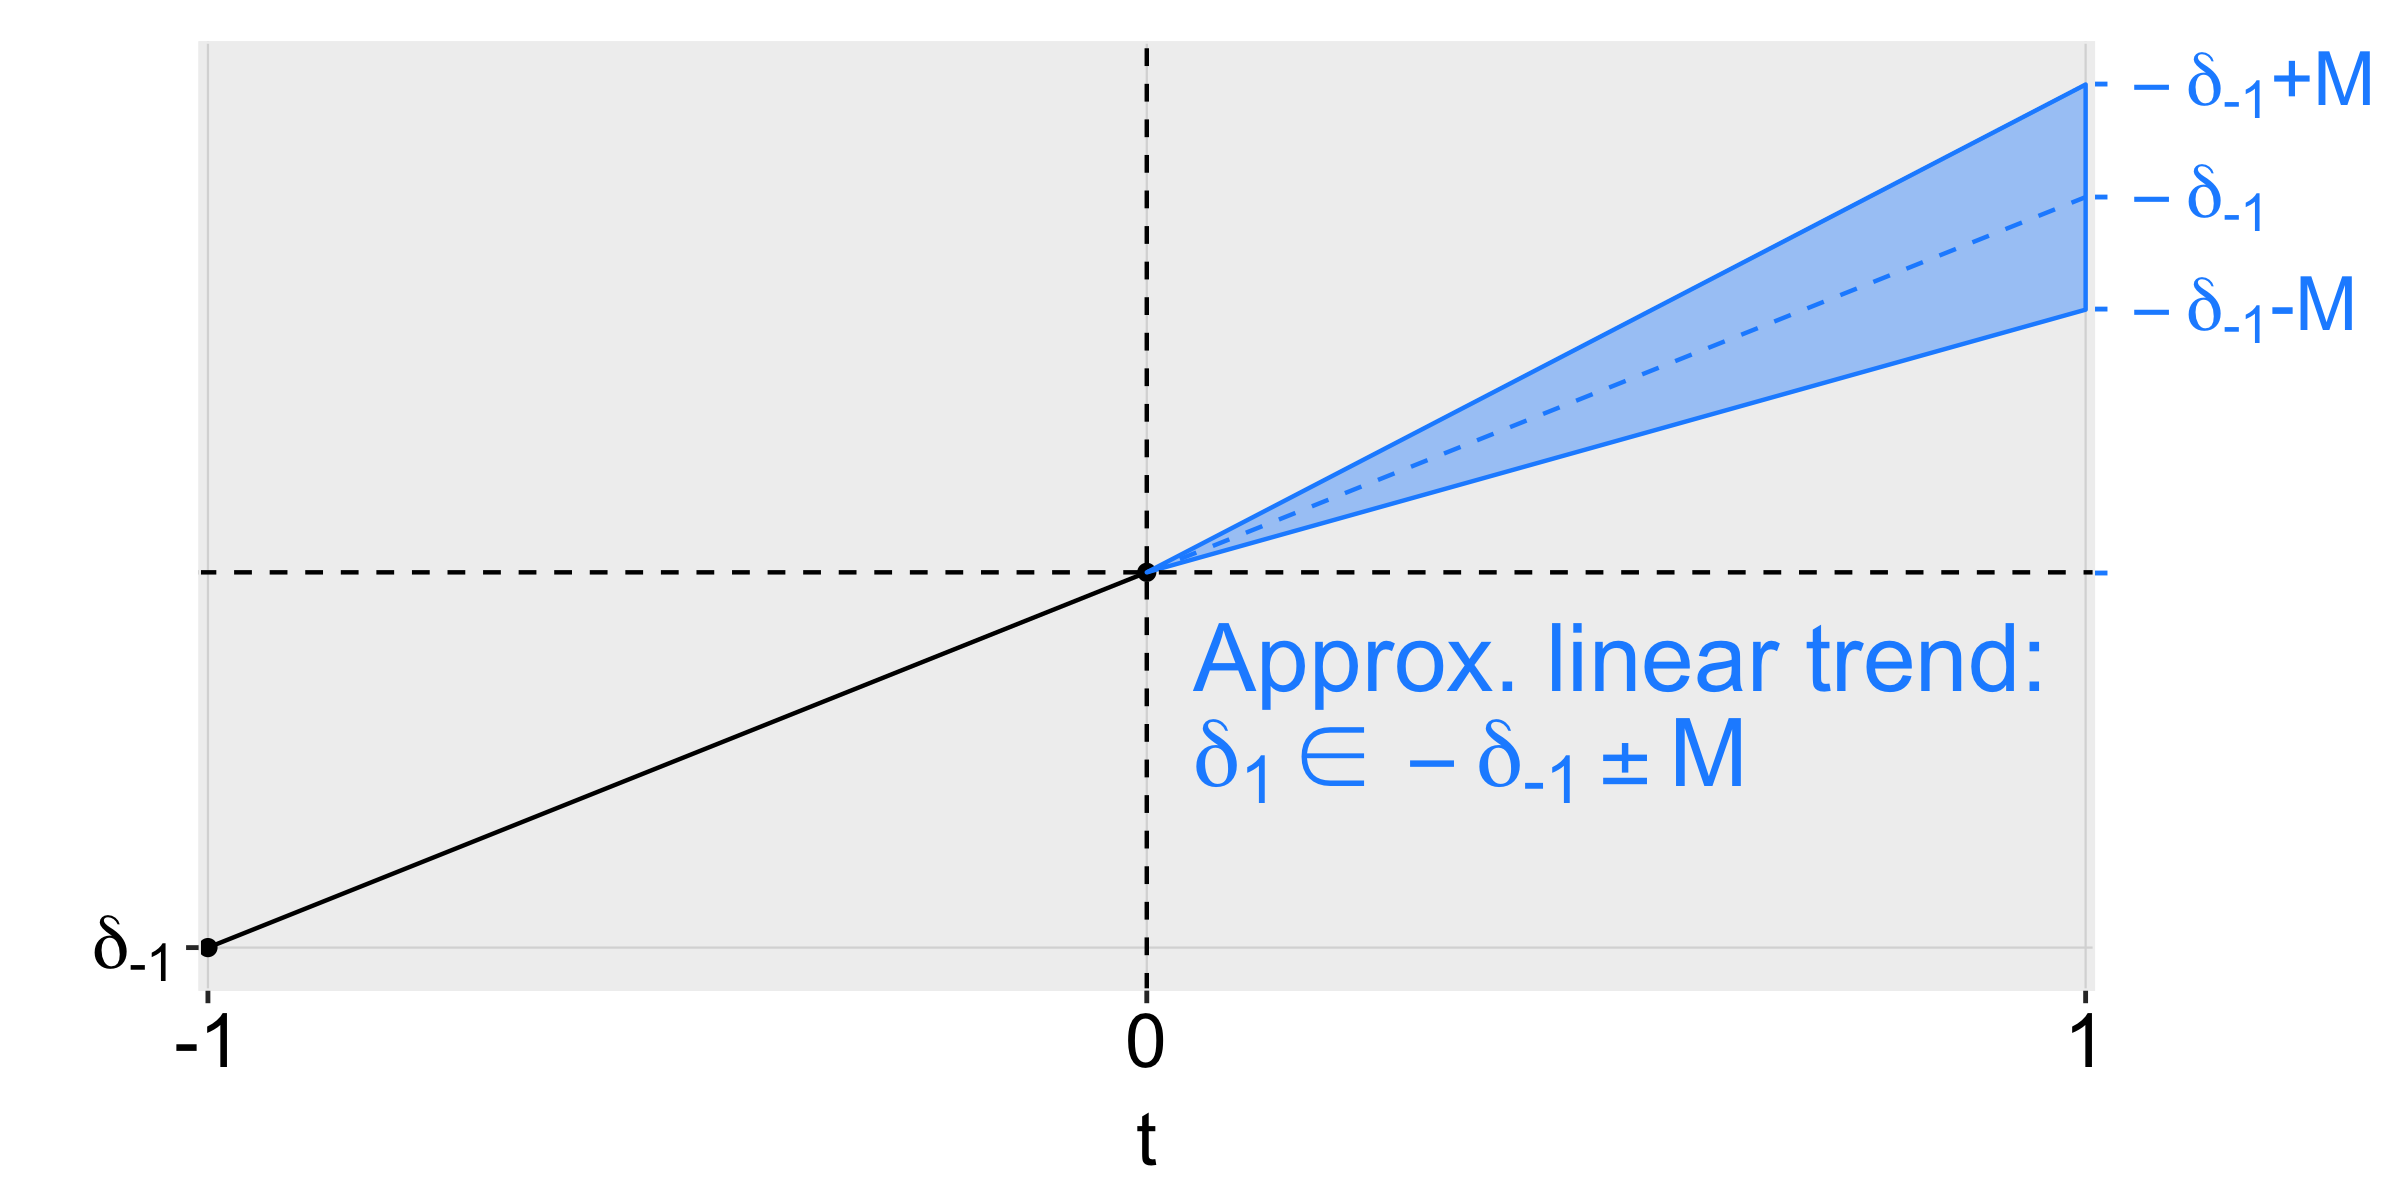
\includegraphics[width = 0.7\textwidth]{Figures/IntuitionPlots/Delta-Examples/deltaSD.png}

\end{frame}



\begin{frame}{Benzarti \& Carloni (2019)}
\begin{wideitemize}
\item
BC study the incidence of a cut in the value-added tax on sit-down restaurants in France.
France reduced the VAT on restaurants from 19.6 to 5.5 percent in July of 2009. 

\item
BC analyze the impact of this change using a difference-in-differences design comparing restaurants to a control group of other market services firms


\begin{equation}
Y_{irt} = \sum_{s = 2004}^{2012} \beta_s \times 1[t = s] \times  D_{ir} + \phi_i + \lambda_t + \epsilon_{irt} , \label{eqn: bc event-study spec}    
\end{equation}

\noindent \begin{itemize}
    \item $Y_{irt}$ = outcome of interest for firm $i$ in region $r$
    \item $D_{ir}$ = indicator if firm $i$ in region $r$ is a restaurant
    \item $\Phi_i, \lambda_t$ = firm and year FEs
\end{itemize}

\item Outcomes of interest include firm profits, prices, wage bill \& employment.\\
We focus on impact on profits in first year after reform.
\end{wideitemize}
\end{frame}

\begin{frame}{Event-study coefficients for log profits}
    \centering
    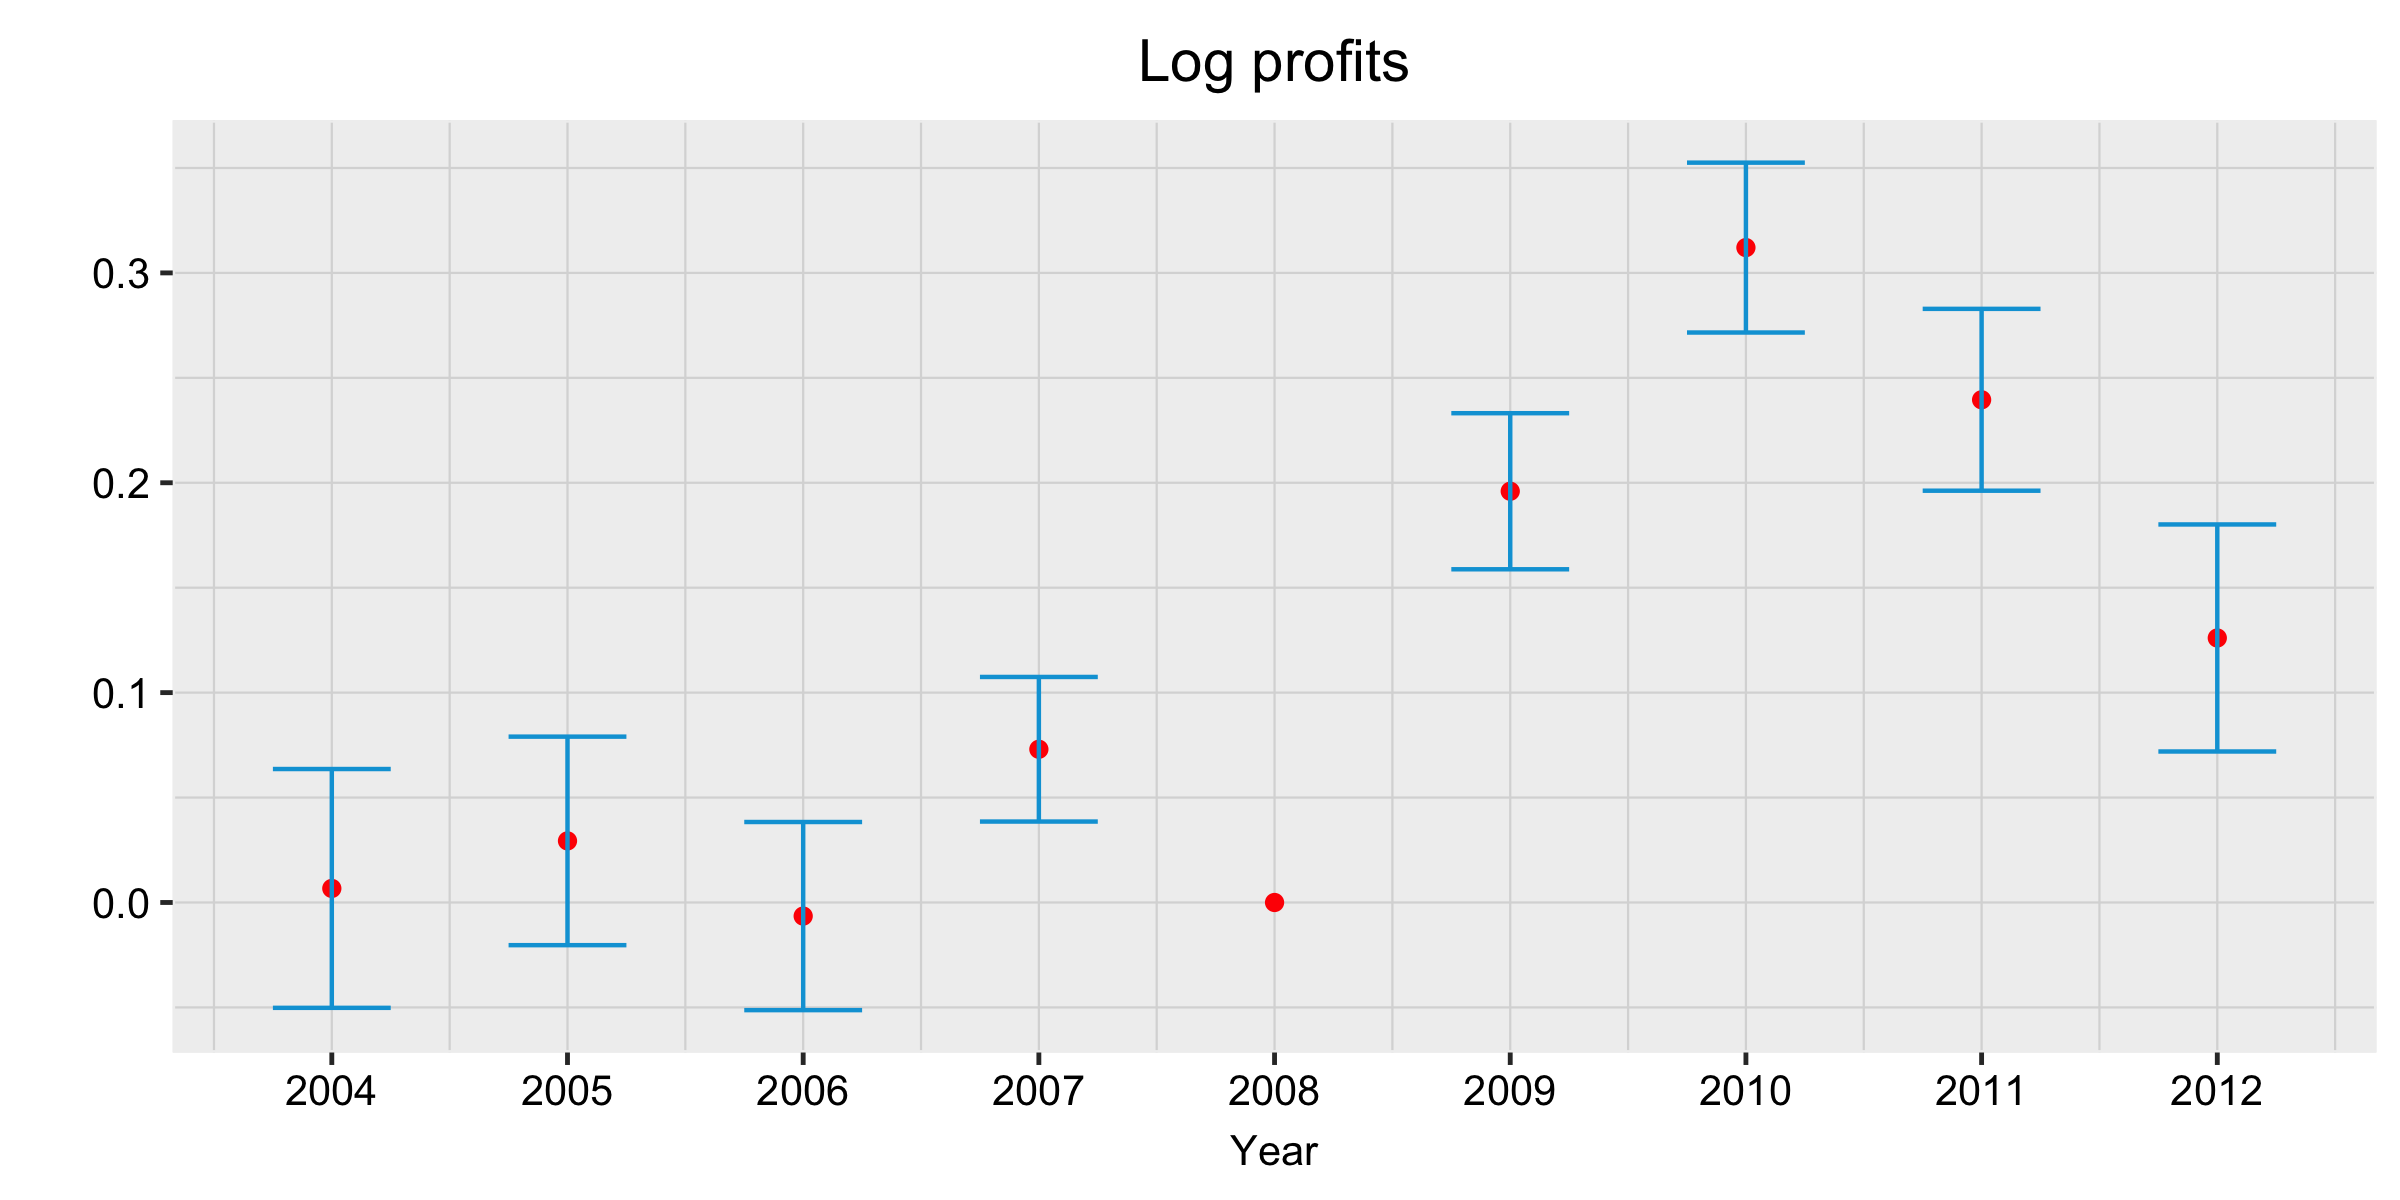
\includegraphics[width = 0.8 \textwidth]{Figures/Benzarti-Carloni/profits-event-study.png}
\end{frame}

\begin{frame}
{\centering
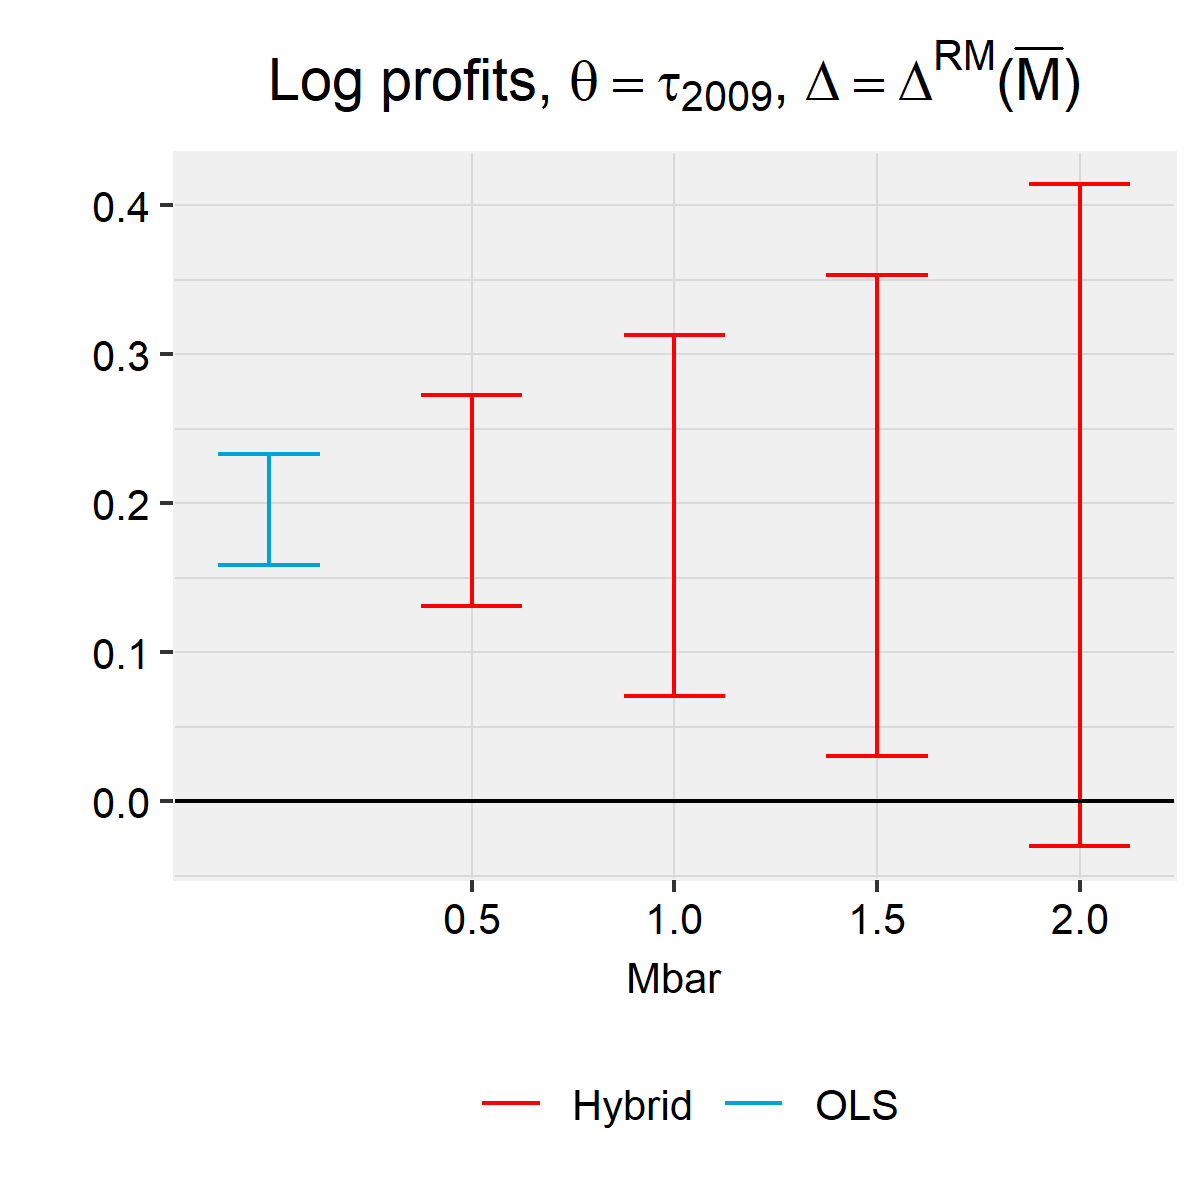
\includegraphics[width = 0.4\linewidth]{Figures/Benzarti-Carloni/sensitivity-MB-profits.png}
}

\begin{itemize}
    \item
    ``Breakdown'' $\bar{M}$ for null effect is $\sim 2$
    
    \item
    Can rule out a null effect unless allow for violations of PT 2x larger than the max in pre-period

\end{itemize}

\end{frame}


\begin{frame}{So to summarize!}
\begin{wideitemize}
    \item
    Tests of pre-trends are intuitive but not a panacea!
    
    \item
    In particular, they may suffer from low power and introduce pre-test bias
    
    \item
    Roth (Forthcoming) and Rambachan and Roth (2022) provide tools for diagnostics and sensitivity analysis
    
    \item
    And these tools play nicely with recent estimators developed for heterogeneous treatment effects; see Pedro Sant'Anna's website for examples!
    
\end{wideitemize}
\end{frame}

\begin{frame}{Other Related Papers}

\begin{wideitemize}

\item
Other bounding exercises \citep{manski_how_2017, ye_negative_2021}

\item
Non-inferiority approaches to pre-testing \citep{bilinski_no_2018, dette_difference--differences_2020}

\item
Impose structure on the confounds \citep{freyaldenhoven_pre-event_2019}
\end{wideitemize}
    
\end{frame}


% \begin{frame}{Wrapping Up}

% \begin{wideitemize}

% \item
% Tests of pre-trends are intuitive but not a panacea!

% \item
% Roth (2021) and Rambachan and Roth (2021) provide tools for diagnostics and sensitivity analysis

% \item
% It's important to incorporate \textit{context-specific} knowledge when using these tools.

% \item
% \textbf{Think about how parallel trends may be violated in your context!}\\
% This puts the ``econ'' back into ``econometrics''
% \end{wideitemize}
    
% \end{frame}


\backupbegin
\appendix


\begin{frame}
\centering
Thank you!
\end{frame}


\begin{frame}{Additional Resources}
\begin{wideitemize}
\item
Roth (2021), ``Pre-test with Caution: Event-study Estimates After Testing for Parallel Trends''
    \begin{itemize}
        \item 
        \href{https://jonathandroth.github.io/assets/files/roth_pretrends_testing.pdf}{Paper}; \href{https://github.com/jonathandroth/pretrends}{\texttt{staggered} package} ; \href{https://github.com/jonathandroth/PretrendsPower\#pretrendspower}{Shiny app}
    \end{itemize}
    
\item
Rambachan and Roth (2022), ``A More Credible Approach to Parallel Trends'''
    \begin{itemize}
        \item 
        \href{https://jonathandroth.github.io/assets/files/HonestParallelTrends_Main.pdf}{Paper}; \href{https://github.com/asheshrambachan/HonestDiD}{\texttt{HonestDiD} package} ; \href{https://github.com/asheshrambachan/HonestDiD/blob/master/doc/HonestDiD_Example.pdf}{Vignette}
    \end{itemize}
\end{wideitemize}
\end{frame}


\begin{frame}[label = power_analysis]{Pre-testing Diagnostics}
\begin{wideitemize}
\item
A ``low-touch'' intervention is to evaluate the likely power/distortions from pre-testing under \textit{context-relevant} violations of parallel trends

\item Enter the \texttt{pretrends} package / Shiny app
\end{wideitemize}
\end{frame}

\begin{frame}
\centering
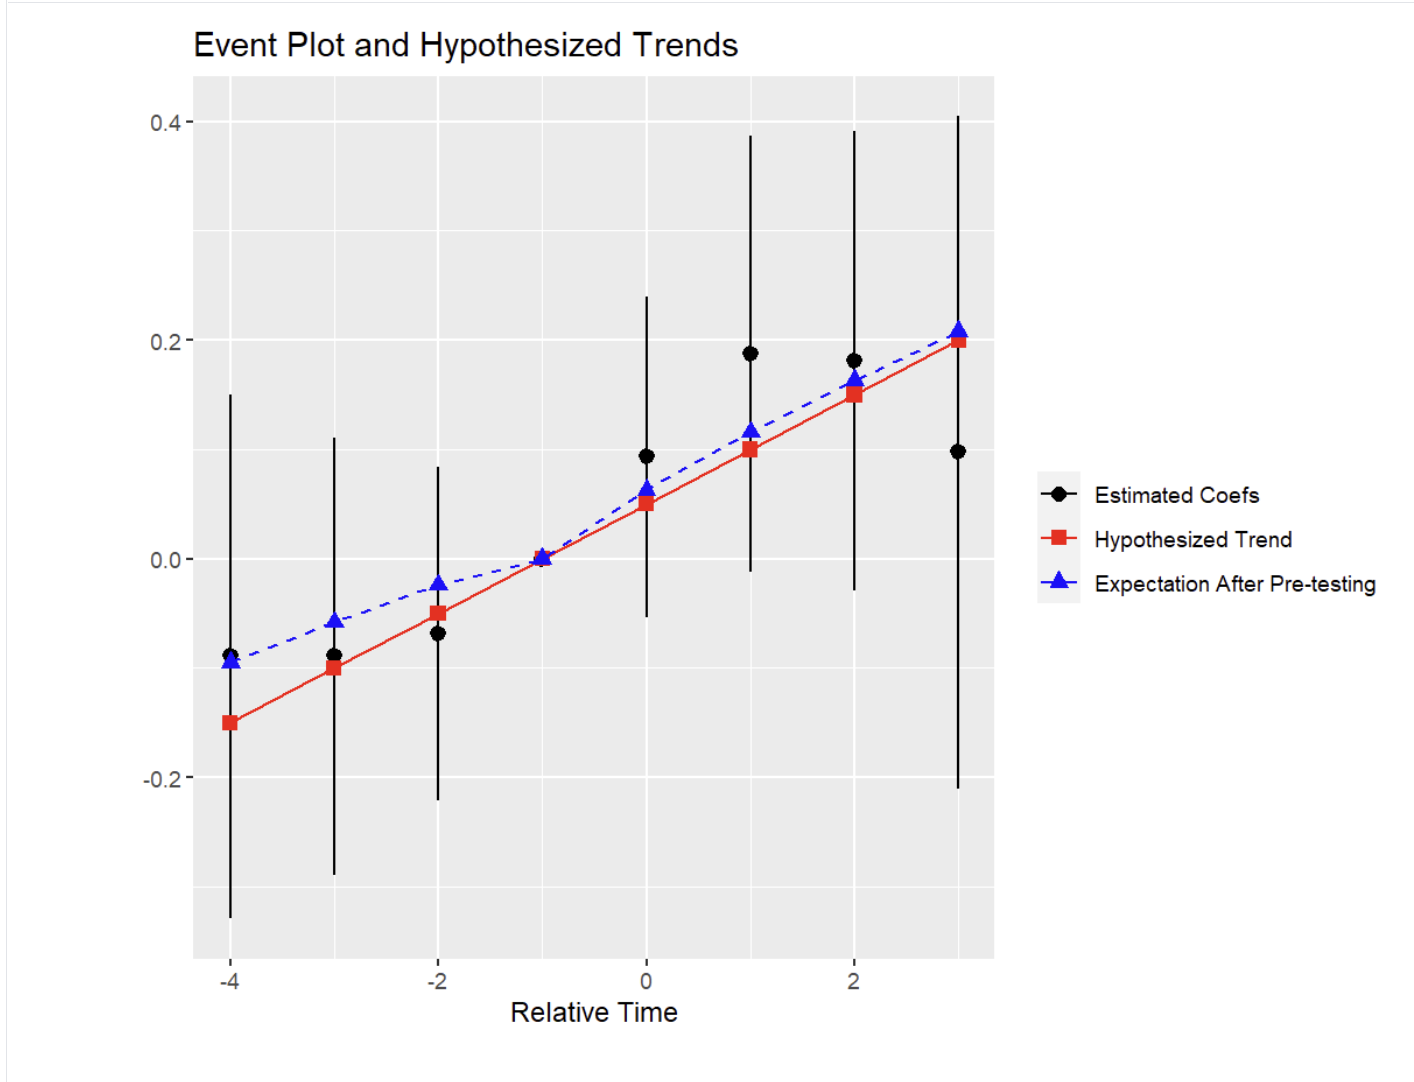
\includegraphics[height = 0.9 \textheight]{Figures/Shiny-Mockup-Graph-Only.png}   
\end{frame}

\begin{frame}
\centering
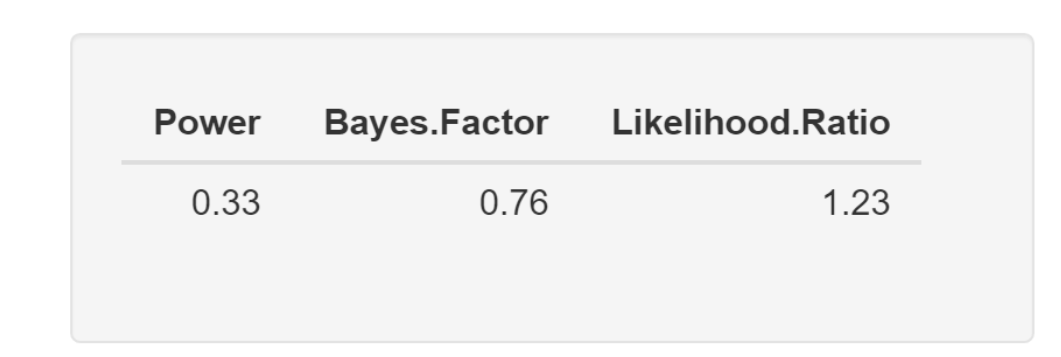
\includegraphics[width = 0.7 \textwidth]{Figures/Shiny-Mockup-Power-Only.png} 
\begin{wideitemize}
\item
\textbf{Power.} Chance find significant pre-trend under hypothesized trend.
\item
\textbf{Bayes Factor.} Relative chance you pass the pre-test under hypothesized trend versus under parallel trends.
\item
\textbf{Likelihood Ratio.} Likelihood of observed pre-trend coefs under hypothesized trend versus under parallel trends.
\end{wideitemize}
\end{frame}

\begin{frame}{Pros and Cons}
\textbf{Pros}
\begin{wideitemize}
    \item
    Very intuitive, easy to visualize.

    \item
    Helps identify when pre-testing may be least effective
    
    \item
    Requires minimal changes from standard practice
\end{wideitemize}

\textbf{Cons}

\begin{wideitemize}
    \item
    Power will always be $<1$, so no guarantee of unbiasedness/correct inference
    
    \item
    Need to specify the hypothesized trend. Will sometimes be difficult to summarize over many of these.
    
    \item
    Still not clear what to do when reject the pre-test.
\end{wideitemize}
    
\end{frame}





\bibliography{Bibliography.bib}
\backupend

\end{document} 